%% GreenMind AI — IEEE Conference Paper (5-Page Target)
%% IEEEtran conference style
%% Compile: pdflatex → bibtex → pdflatex × 2  (or use overleaf)
\documentclass[conference]{IEEEtran}
\IEEEoverridecommandlockouts
\usepackage{cite}
\usepackage{amsmath,amssymb}
\usepackage{graphicx}
\usepackage{booktabs}
\usepackage{url}
\usepackage{microtype}
\usepackage[T1]{fontenc}
\usepackage[hidelinks]{hyperref}

% ── Tight list spacing ────────────────────────────────────────────────────────
\usepackage{enumitem}
\setlist[itemize]{noitemsep,topsep=2pt,leftmargin=*}
\setlist[enumerate]{noitemsep,topsep=2pt,leftmargin=*}

\title{GreenMind AI: A Multi-Metric Forecasting and Decision-Support\\
Platform for Cloud GreenOps}

\author{%
  \IEEEauthorblockN{Anonymous Submission Draft}\\
  \IEEEauthorblockA{%
    \textit{[Author affiliations to be inserted for camera-ready submission]}\\
    \texttt{[contact@institution.edu]}
  }
}

\begin{document}
\maketitle

%% ── ABSTRACT ─────────────────────────────────────────────────────────────────
\begin{abstract}
Modern cloud operations require optimizing resource utilization, cost, and
environmental footprint simultaneously. We present GreenMind AI, an
open-source decision-support prototype that integrates five one-hour-ahead
gradient-boosted forecasters, a five-domain multi-agent analysis engine
(Cost, Performance, Sustainability, Security, Reliability), deterministic
conflict arbitration, a non-destructive Digital Twin simulator, and an
eight-tool explainable AI copilot. Evaluation on a deterministic 60-day
synthetic dataset (5,756 records; strict 80/20 chronological split:
$N_{\text{train}}=4{,}604$, $N_{\text{test}}=1{,}152$) shows MAE
improvements of 25.4\%--45.4\% over a one-hour persistence baseline across
five targets. Our audit reveals a stored rolling-mean baseline reflects a
one-step-ahead (15-min) prediction rather than the correct four-step horizon;
the true four-step rolling baseline achieves higher error than persistence
(e.g., 7.263\% vs.\ 6.500\% CPU MAE) due to diurnal phase shift. We
document that all evaluations originate from synthetic generator equations,
live cloud connectors are validated in simulation only, and direct
remediation is guarded by an HTTP~501 boundary. GreenMind AI provides
integrated decision-support architecture; synthetic accuracy must not be
conflated with verified production savings.
\end{abstract}

\begin{IEEEkeywords}
cloud computing; workload forecasting; gradient boosting; carbon-aware
computing; multi-agent systems; digital twin; explainability; GreenOps.
\end{IEEEkeywords}

%% ── I. INTRODUCTION ─────────────────────────────────────────────────────────
\section{Introduction}
Cloud data centers account for a rising share of global electricity
consumption, pushing providers and tenants toward GreenOps and FinOps
disciplines~\cite{r4,r6}. Proactive telemetry forecasting supports
right-sizing, autoscaling, and carbon-aware job scheduling, but high
prediction accuracy on historical data does not guarantee realized savings,
carbon abatement, or service-level preservation in live
systems~\cite{r3,r8}.

Existing platforms treat cost, performance, sustainability, and reliability
as siloed concerns. When agents generate conflicting recommendations---e.g.,
scale-up for performance versus scale-down for cost---operators lack
transparent arbitration. Likewise, evaluating proposed changes without
touching live infrastructure requires a safe simulation layer.

GreenMind AI addresses these gaps by unifying (i) multi-metric gradient
boosted forecasting, (ii) multi-domain agent orchestration via a state
graph, (iii) deterministic conflict resolution with explicit audit logs,
(iv) a non-destructive Digital Twin simulator, and (v) an eight-tool
AI copilot grounded in live application state.

\textbf{Contributions:}
\begin{enumerate}
  \item End-to-end software architecture linking telemetry ingestion,
        multi-metric forecasting, multi-agent arbitration, Digital Twin
        simulation, and decision-support interfaces.
  \item Verified forecasting performance on five targets, with a baseline
        alignment audit identifying a 15-min vs.\ 1-h horizon discrepancy
        in the stored rolling baseline.
  \item Explicit demarcation of empirical evidence boundaries: synthetic
        data provenance, unverified live connectors, and the HTTP~501
        live-remediation safety guard.
\end{enumerate}

%% ── II. RELATED WORK ─────────────────────────────────────────────────────────
\section{Related Work}
Calheiros et al.~\cite{r7} demonstrated proactive cloud provisioning with
ARIMA, showing that predictive scaling reduces QoS violations compared to
reactive policies. Friedman's Gradient Boosting Machine~\cite{r1} constructs
additive tree models well-suited to structured tabular lag features. Rossi
et al.~\cite{r3} evaluated probabilistic LSTMs on Google and Alibaba cluster
traces, highlighting that point forecasts miss operational uncertainty and
that accuracy degrades under transfer learning across providers.

For time-series evaluation methodology, Bergmeir et al.~\cite{r2} showed
that chronological holdout remains standard practice to avoid forward leakage.
In sustainability, Henderson et al.~\cite{r4} established energy and carbon
reporting standards for ML; Lannelongue et al.~\cite{r5} formalized the
Green Algorithms carbon calculation framework. Radovanovic et al.~\cite{r6}
deployed carbon-aware scheduling at Google data centers using day-ahead
grid predictions. Dodge et al.~\cite{r8} quantified operational carbon
intensity across cloud instance types, confirming region selection and
temporal scheduling as primary levers.

GreenMind AI extends these foundations to a unified prototype with
multi-domain agent orchestration and Digital Twin simulation, but evaluates
exclusively on synthetic telemetry rather than measured traces.

%% ── III. ARCHITECTURE ────────────────────────────────────────────────────────
\section{Platform Architecture and Implementation}

\begin{figure}[t]
  \centering
  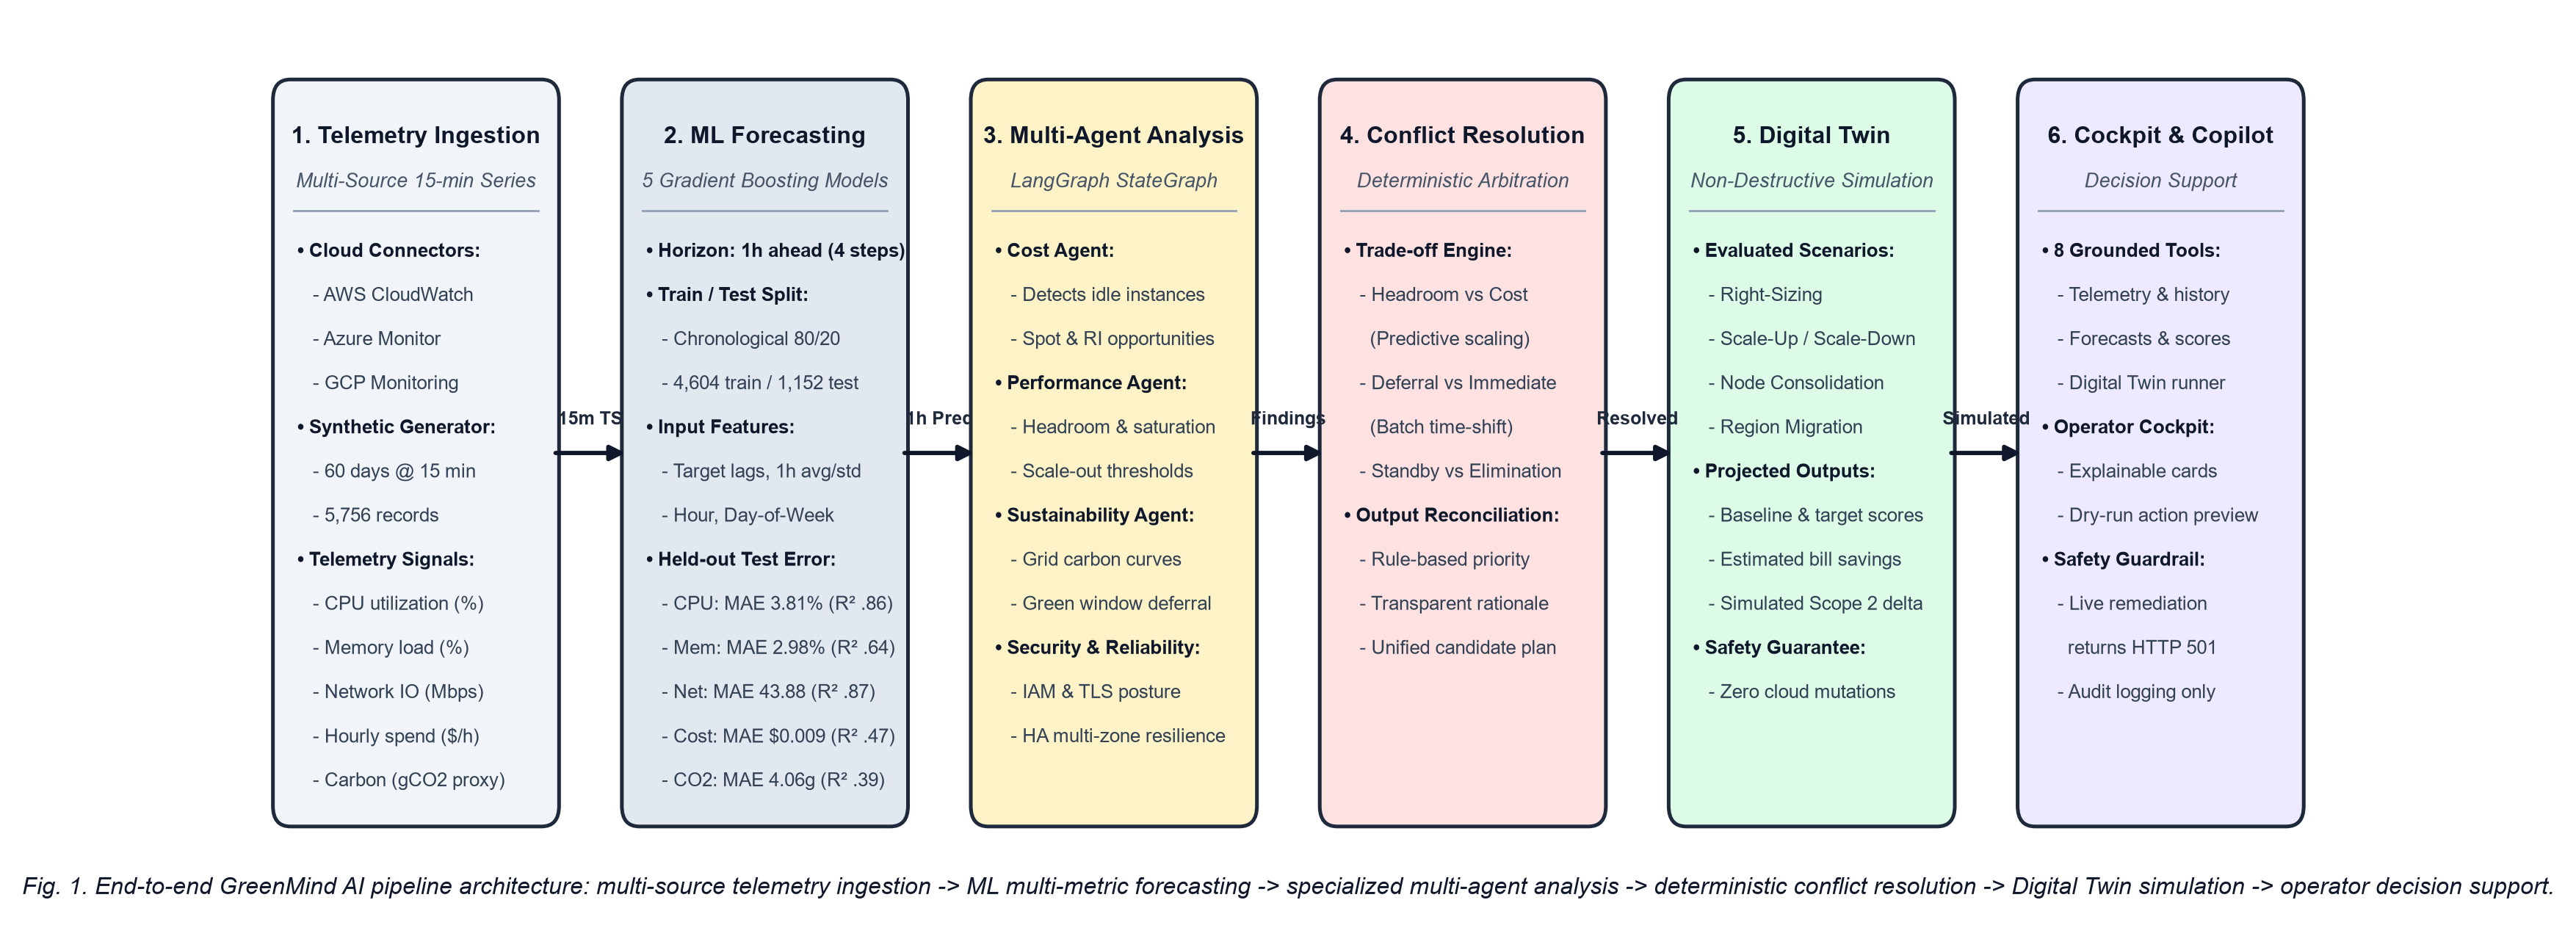
\includegraphics[width=\columnwidth]{greenmind_architecture.png}
  \caption{GreenMind AI end-to-end pipeline: telemetry ingestion
  $\!\to\!$ ML forecasting $\!\to\!$ multi-agent analysis $\!\to\!$
  conflict resolution $\!\to\!$ Digital Twin simulation $\!\to\!$
  operator decision support.}
  \label{fig:arch}
\end{figure}

Fig.~\ref{fig:arch} illustrates the six interconnected components.

\subsection{Telemetry Ingestion and Service Layer}
The backend (FastAPI, Python~3.12; SQLite/PostgreSQL) ingests five signals
at 15-min intervals: CPU~(\%), memory~(\%), network traffic~(Mbps), compute
cost~(USD/h), and a synthetic carbon emissions proxy~(gCO$_2$/15-min).
Connector modules target AWS~CloudWatch (\texttt{boto3}), Azure Monitor REST
APIs, and GCP Cloud Monitoring~v3; each falls back to a deterministic
synthetic generator when live credentials are absent.

\subsection{Multi-Metric ML Predictor}
Five independent \texttt{GradientBoostingRegressor} models (scikit-learn)
forecast one hour ahead ($\Delta=4\times15$~min). Shared hyperparameters:
150 estimators, max depth~3, learning rate~0.08, \texttt{random\_state=42}.
Features are constructed to be strictly backward-looking:

\begin{itemize}
  \item \textbf{CPU/Memory/Network}: current value $y_t$, hour of day,
        day of week, one-hour rolling mean
        $\mu_{t,4}=\tfrac{1}{4}\sum_{i=0}^{3}y_{t-i}$, and rolling
        standard deviation $\sigma_{t,4}$.
  \item \textbf{Cost}: current CPU, memory, cost $y_t$, hour, day.
  \item \textbf{Carbon proxy}: regional grid intensity
        (gCO$_2$/kWh), hour, day, CPU.
\end{itemize}

Anomaly detection flags predictions with z-score $>2.5$ against running
metric statistics.

\subsection{Multi-Agent Analysis Engine}
Five specialized agents execute as a LangGraph \texttt{StateGraph}:
\textbf{CostAgent} (right-sizing, Spot/RI recommendations),
\textbf{PerformanceAgent} (saturation thresholds, autoscaling triggers),
\textbf{SustainabilityAgent} (green scheduling windows),
\textbf{SecurityAgent} (IAM, TLS, port auditing),
\textbf{ReliabilityAgent} (multi-AZ topology, backup RPO).
LangGraph is unavailable, agents execute sequentially with deduplication.

\subsection{Deterministic Conflict Resolution}
Opposing recommendations trigger explicit arbitration:
\begin{itemize}
  \item \textbf{Performance vs.\ Cost}: $35\%\!\le\!$CPU$\!<\!75\%$
        $\Rightarrow$ right-size with predictive autoscaling (60-s buffer).
  \item \textbf{Reliability vs.\ Cost} ($\text{CPU}<35\%$): downsize
        while preserving automated horizontal failover.
  \item \textbf{Carbon deferral vs.\ Execution}: non-critical batches
        shifted to 01:00--06:00~UTC green windows; interactive APIs
        remain on immediate paths.
\end{itemize}
Each resolution emits an audit record with competing agents, rationale,
and confidence score (0.87--0.92).

\subsection{Digital Twin Simulator}
Five non-destructive scenarios: \textsc{Right-Size},
\textsc{Scale-Up/Down}, \textsc{Consolidate}, \textsc{Region~Migration}.
The engine applies parameterized deltas to a state snapshot and
recomputes a composite Optimization Score (0--100). All outputs carry
\texttt{is\_simulated=True} and an explicit
\texttt{"SIMULATED / ESTIMATED"} label.

\subsection{AI Copilot and Safe Remediation Boundary}
Eight grounded tools: \texttt{get\_cloud\_metrics},
\texttt{get\_history}, \texttt{get\_predictions},
\texttt{get\_cost\_analysis}, \texttt{get\_carbon\_analysis},
\texttt{get\_recommendations}, \texttt{get\_cloud\_health},
\texttt{run\_digital\_twin\_simulation}. Non-dry-run remediation calls
return \texttt{HTTP~501 Not Implemented}; rollback likewise. Dry-run mode
logs simulated audit events without mutating cloud state.

%% ── IV. EXPERIMENTAL METHODOLOGY ────────────────────────────────────────────
\section{Experimental Methodology}

\subsection{Synthetic Dataset}
\texttt{generate\_dataset.py} produces 5,760 observations at 15-min
intervals starting 2026-06-01 (seed~42). CPU follows:
\begin{equation}
  \text{CPU}_t = \mathrm{clip}\!\left(
    35 + 30\sin^2\!\!\left(\tfrac{h_t-7}{24}2\pi\right)\cdot W_t
    + \tau_t + \epsilon_t,\;2,\,98
  \right)
\end{equation}
where $W_t\!=\!0.7$ on weekends, $\tau_t\!\in\![0,5]\%$ is a linear trend,
and $\epsilon_t\!\sim\!\mathcal{N}(0,16)$.
Memory adds a [0,~8]\% drift (simulated memory leak). Network follows
$300+400\sin^2(\cdot)$~Mbps (peak at~09:00). Cost scales with CPU on an
AWS \texttt{m5.xlarge} baseline (\$0.192/h).

\subsection{Carbon Target Formulation}
Regional grid intensity $I(h_t)$ is looked up from an hourly profile
(\texttt{us-east}: 320--470~gCO$_2$/kWh). Assuming server power draw
$P=0.35$~kW and step size $\Delta t=0.25$~h, the target is:
\begin{equation}
  C_t = \mathrm{clip}\!\left(I(h_t)\cdot P\cdot\Delta t
        + \mathcal{N}(0,25),\;0,\,500\right)
  \;\;[\text{gCO}_2/\text{15-min}]
\end{equation}
This proxy excludes dynamic PUE, server power states, and Scope~3 emissions.

\subsection{Split and Baselines}
Targets are shifted $\Delta=4$ steps; the trailing 4 rows are dropped,
yielding 5,756 aligned records.  An 80/20 chronological split gives
$N_\text{train}=4{,}604$ (48 days) and $N_\text{test}=1{,}152$ (12 days).
No shuffling is performed.

Two baselines are evaluated:
\begin{enumerate}
  \item \textbf{Persistence} ($\hat{y}_{t+4}=y_t$): forecast-origin value.
  \item \textbf{Rolling Mean}: the repository's \texttt{evaluate\_rolling\_mean}
        in \texttt{baseline.py} computes
        $\hat{y}_{t+1}=\mu_{t,4}$ on unshifted test data ($N=1{,}148$),
        effectively a 15-min-ahead prediction.  The \emph{true} four-step
        rolling baseline from origin $t$ yields higher error
        (e.g., CPU: 7.263\% vs.\ stored 4.622\%).
\end{enumerate}

Metrics: MAE, RMSE, $R^2$, and
$\text{Gain}=100\!\times\!(1-\text{MAE}_\text{model}/\text{MAE}_\text{persist.})$.

%% ── V. RESULTS ───────────────────────────────────────────────────────────────
\section{Experimental Results}

\begin{table*}[t]
  \caption{Verified Test-Set Metrics ($N=1{,}152$). Persistence: $\hat{y}_{t+4}=y_t$.
  Stored Roll-4: repository 1-step moving average on unshifted data.
  True Roll-4: four-step-ahead rolling mean from origin $t$.}
  \label{tab:results}
  \centering
  \footnotesize
  \setlength{\tabcolsep}{5pt}
  \begin{tabular}{lrrrrrrr}
    \toprule
    \textbf{Target} & \textbf{MAE} & \textbf{RMSE} & \textbf{$R^2$}
      & \textbf{Persist.\ MAE} & \textbf{Stored Roll-4} & \textbf{True Roll-4}
      & \textbf{Gain (\%)} \\
    \midrule
    CPU Utilization (\%)          & 3.809 & 4.811 & 0.855 & 6.500 & 4.622 & 7.263 & 41.4 \\
    Memory Utilization (\%)       & 2.979 & 3.704 & 0.636 & 3.996 & 3.025 & 4.153 & 25.4 \\
    Network Traffic (Mbps)        & 43.876 & 55.328 & 0.871 & 80.346 & 56.727 & 90.816 & 45.4 \\
    Hourly Cost (USD/h)           & 0.009 & 0.011 & 0.474 & 0.013 & 0.010 & N/A & 29.7 \\
    Carbon Proxy (gCO$_2$/15-min) & 4.061 & 5.087 & 0.391 & 5.846 & 4.571 & N/A & 30.5 \\
    \bottomrule
  \end{tabular}
\end{table*}

Table~\ref{tab:results} reports fully verified held-out metrics reproduced
identically by re-running \texttt{train.py} (seed~42, 6.4~s wall-clock).

Gradient boosted regressors outperform the forecast-origin persistence
baseline on all five targets. Relative MAE gains range from 25.4\%
(memory, lowest diurnal amplitude) to 45.4\% (network, highest).
CPU and network achieve the best fit ($R^2=0.855$ and $0.871$,
respectively), reflecting the models' ability to capture the generator's
sinusoidal patterns. Cost ($R^2=0.474$) and carbon ($R^2=0.391$) show
lower explained variance due to additive observation noise ($\sigma=0.01$
and $\sigma=5$) on relatively small base values, creating irreducible
noise floors.

\textbf{Feature importances} (extracted from tree structures):
CPU prediction is dominated by the current lag (69.4\%), hour of day (22.3\%),
day of week (4.8\%), and rolling mean (3.3\%). Carbon prediction is dominated
by regional grid intensity (71.1\%), hour (20.0\%), and CPU (8.5\%), which
mirrors the generator's $C_t = I(h_t)\cdot E + \epsilon$ construction.

\textbf{Baseline alignment audit}: The repository's stored
\texttt{rolling\_mae} evaluates a one-step-ahead (15-min) moving average on
unshifted test observations, achieving low error due to high lag-1
autocorrelation ($e.g.,$ CPU: 4.622\%). The true four-step rolling baseline
from forecast origin performs \emph{worse} than persistence for CPU
(7.263\% vs.\ 6.500\%), memory (4.153\% vs.\ 3.996\%), and network
(90.816 vs.\ 80.346~Mbps) because the moving average lags behind diurnal
transitions. Gradient boosted models decisively outperform both baselines
under correct horizon alignment.

%% ── VI. DISCUSSION ───────────────────────────────────────────────────────────
\section{Discussion and Limitations}

\subsection{Synthetic vs.\ Real Generalization}
High $R^2$ on CPU and network reflects recovery of the smooth sinusoidal
generator formulas in \texttt{generate\_dataset.py}. Real hyperscale traces
(Google~Borg, Alibaba cluster, Azure Functions) exhibit heavy-tailed job
distributions, sudden preemptions, and non-stationary distribution shifts
absent from the synthetic series~\cite{r3}. Reported metrics establish
\emph{synthetic benchmark performance only}.

\subsection{Documented Limitations}
\begin{enumerate}
  \item \textbf{Data provenance}: all evaluations derive from a single
        generator configuration (seed~42, 60-day, \texttt{us-east}).
  \item \textbf{Recursive multi-step inconsistency}: \texttt{forecast\_multi\_step}
        in \texttt{predictor.py} applies 5-min recursive steps using
        models trained on 1-h direct shifts, and feeds back carbon output
        ($\sim$30--40~gCO$_2$/15-min) into the \texttt{carbon\_intensity}
        input that was trained on grid values ($\sim$350--450~gCO$_2$/kWh),
        an $\approx$10$\times$ scale mismatch.
  \item \textbf{Live connector validation}: AWS, Azure, and GCP connectors
        fall back to synthetic data in the test environment; end-to-end
        live polling was not validated against real accounts.
  \item \textbf{No live remediation}: all non-dry-run and rollback
        endpoints return HTTP~501; reported Digital Twin savings
        (\$864/month illustrative) are static model projections.
  \item \textbf{Carbon accounting}: the proxy assumes a fixed 350~W server,
        excluding dynamic power states, PUE variations, cooling overhead,
        and embodied lifecycle emissions~\cite{r5}.
\end{enumerate}

%% ── VII. CONCLUSION ──────────────────────────────────────────────────────────
\section{Conclusion}
GreenMind AI implements a complete prototype coupling five one-hour-ahead
gradient boosted forecasters with five-domain multi-agent orchestration,
deterministic conflict arbitration, Digital Twin simulation, and an
eight-tool AI copilot. On a 60-day synthetic benchmark, MAE improves
25.4\%--45.4\% over persistence.  These results reflect synthetic-generator
learning; production validation requires open cluster traces, real-time
grid intensity feeds (Electricity Maps / WattTime), recursive horizon
alignment refactoring, and end-to-end testing against isolated canary cloud
accounts before autonomous operational claims can be substantiated.

%% ── REFERENCES ───────────────────────────────────────────────────────────────
\begin{thebibliography}{00}

\bibitem{r1}
  J.~H. Friedman, ``Greedy function approximation: A gradient boosting
  machine,'' \emph{The Annals of Statistics}, vol.~29, no.~5,
  pp.~1189--1232, Oct.~2001, doi:~\href{https://doi.org/10.1214/aos/1013203451}{10.1214/aos/1013203451}.

\bibitem{r2}
  C.~Bergmeir, R.~J. Hyndman, and B.~Koo, ``A note on the validity of
  cross-validation for evaluating autoregressive time series prediction,''
  \emph{Computational Statistics \& Data Analysis}, vol.~120,
  pp.~70--83, Apr.~2018, doi:~\href{https://doi.org/10.1016/j.csda.2017.11.003}{10.1016/j.csda.2017.11.003}.

\bibitem{r3}
  A.~Rossi, A.~Visentin, D.~Carraro, S.~Prestwich, and K.~N. Brown,
  ``Forecasting workload in cloud computing: Towards uncertainty-aware
  predictions and transfer learning,'' \emph{Cluster Computing}, vol.~28,
  art. no.~258, 2025, doi:~\href{https://doi.org/10.1007/s10586-024-04933-2}{10.1007/s10586-024-04933-2}.

\bibitem{r4}
  P.~Henderson \emph{et al.}, ``Towards the systematic reporting of the
  energy and carbon footprints of machine learning,''
  \emph{Journal of Machine Learning Research}, vol.~21, no.~248,
  pp.~1--43, 2020.

\bibitem{r5}
  L.~Lannelongue, J.~Grealey, and M.~Inouye, ``Green algorithms:
  Quantifying the carbon footprint of computation,''
  \emph{Advanced Science}, vol.~8, no.~12, art. no.~2100707, 2021,
  doi:~\href{https://doi.org/10.1002/advs.202100707}{10.1002/advs.202100707}.

\bibitem{r6}
  A.~Radovanovic \emph{et al.}, ``Carbon-aware computing for data centers,''
  \emph{IEEE Trans.\ Power Systems}, vol.~38, no.~2, pp.~1270--1280,
  Mar.~2023, doi:~\href{https://doi.org/10.1109/TPWRS.2022.3173250}{10.1109/TPWRS.2022.3173250}.

\bibitem{r7}
  R.~N. Calheiros, E.~Masoumi, R.~Ranjan, and R.~Buyya, ``Workload
  prediction using ARIMA model and its impact on cloud applications' QoS,''
  \emph{IEEE Trans.\ Cloud Computing}, vol.~3, no.~4, pp.~449--458,
  Oct.--Dec.~2015, doi:~\href{https://doi.org/10.1109/TCC.2014.2350475}{10.1109/TCC.2014.2350475}.

\bibitem{r8}
  J.~Dodge \emph{et al.}, ``Measuring the carbon intensity of AI in cloud
  instances,'' in \emph{Proc.\ ACM FAccT '22}, Seoul, Republic of Korea,
  2022, pp.~1536--1546, doi:~\href{https://doi.org/10.1145/3531146.3533147}{10.1145/3531146.3533147}.

\bibitem{r9}
  Pratham-stack-coder, ``GreenMind-AI repository,'' GitHub, 2026. [Online].
  Available: \url{https://github.com/Pratham-stack-coder/GreenMind-AI}.

\end{thebibliography}

\end{document}
